\documentclass{article}

% set font encoding for PDFLaTeX, XeLaTeX, or LuaTeX
\usepackage{ifxetex,ifluatex}
\newif\ifxetexorluatex
\ifxetex
  \xetexorluatextrue
\else
  \ifluatex
    \xetexorluatextrue
  \else
    \xetexorluatexfalse
  \fi
\fi

\ifxetexorluatex
  \usepackage{fontspec}
\else
  \usepackage[T1]{fontenc}
  \usepackage[utf8]{inputenc}
  \usepackage{lmodern}
\fi

\usepackage{hyperref}
\usepackage{amsmath} % para pmatrix
\usepackage{color}
\usepackage{graphicx}

\setlength{\parindent}{0pt}% sangria


\title{Redes neuronales}
\author{Aure}

% Enable SageTeX to run SageMath code right inside this LaTeX file.
% http://mirrors.ctan.org/macros/latex/contrib/sagetex/sagetexpackage.pdf
% \usepackage{sagetex}

\begin{document}
\maketitle

\section{Red Neuronal}
Se conoce como red neuronal a un conjunto de capas de neuronas (variables con valores en $[0,1]$) conectadas mediante pesos (coeficientes de ponderación). El valor de las neuronas de la primera capa es el valor del input del programa. Los valores de las neuronas de las siguientes capas provienen de las capas anteriores, su valores son una suma ponderada por los pesos de las neuronas de la capa anterior evaluada en una función de manera que el valor vuelve a estar en $[0,1] $. Además cada neurona tendrá un umbral de activación para controlar donde se quiere establecer el "cero" de la activación.\\

Finalmente el programa devolverá un output que serán los valores de la última capa de neuronas. Si los valores no son como se esperan entonces tras cada prueba deberán cambiarse los pesos y umbrales. De manera que "aprender" en realidad es encontrar pesos y umbrales más adecuados.\\

El resultado final será un programa que se auto-refina esos parámetros automáticamente a través de ejemplos (entrenos) mediante ensayo-error.
\subsection{Activaciones de las neuronas, función sigmoide}
La red tendrá $c$ capas y cada capa tendrá $n_k$ neuronas $1\leq k\leq c $. Cada neurona está conectada con cada una de las neuronas de la siguiente capa.\\
A la $i$-ésima neurona $1\leq i\leq n_k $ de la capa $k$ la denotaremos por $a_i^{(k)} $. El umbral o peso de dicha neurona la denotaremos por $u_i^{(k)}$. (A veces se denota como $b_i^{(k)} $ por el inglés bias).\\
La conexión de la $i$-ésima neurona $1\leq i\leq n_k$ de la capa $k$ con la neurona $j$-ésima $1\leq j\leq n_{k+1}$ de a capa $k+1$ la denotaremos por $\omega^{(k)}_{ji} $.\\
Todos estos parámetros (pesos y umbrales) se inicializarán con valores aleatorios comprendidos entre $0$ y $1$.\\

Consideremos la siguiente función, conocida como sigmoide
$$f(x)=\frac1{1+e^{-x}}\in (0,1) $$
que cumple que 
$$f'(x)=f(x)\cdot (1-f(x)) $$
\textcolor{red}{Se dice que ahora se usa mejor la función ReLU$(x)=$max$(0,x) $}.\\
El output de la capa $k=1$ es simplemente el input del programa y para $k>1$ tendremos que
$$a^{(k)}_i=f(\sum_{j=1}^{n_{k-1}} w^{(k-1)}_{ij}a^{(k-1)}_j+u^{(k-1)}_i) $$

Por lo general podemos pensarlo como \\
\textcolor{red}{creo k me he colado con la capa de las $\omega$,deberia ser k y no k-1}
$$
\begin{pmatrix}
a^{(k)}_1 \\
a^{(k)}_2 \\
\vdots \\
a^{(k)}_{n_k} \\
\end{pmatrix}
=f\left(
\begin{pmatrix}
w^{(k-1)}_{11} & w^{(k-1)}_{12} \cdots w^{(k-1)}_{1n_{k-1}}\\
w^{(k-1)}_{21} & w^{(k-1)}_{22} \cdots w^{(k-1)}_{2n_{k-1}}\\
\vdots   & \ddots  \\
w^{(k-1)}_{{n_k}1} & w^{(k-1)}_{{n_k}2} \cdots w^{(k-1)}_{{n_k}n_{k-1}}\\
\end{pmatrix} 
\begin{pmatrix}
a^{(k-1)}_1 \\
a^{(k-1)}_2 \\
\vdots \\
a^{(k-1)}_{n_{k-1}} \\
\end{pmatrix}
+
\begin{pmatrix}
u^{(k-1)}_1 \\
u^{(k-1)}_2 \\
\vdots \\
u^{(k-1)}_{n_{k-1}} \\
\end{pmatrix}\right)$$
y por lo tanto en forma matricial nos quedaría
$$a^{(k)}=f(\omega^{(k-1)}a^{(k-1)}+b^{(k-1)}) $$
Observamos que aquí queda justificado el orden de los subíndices $ji$ de la definición de los pesos, ya que si no la matriz anterior tendría que estar traspuesta.
\subsection{Última capa de neuronas, función coste y descenso del gradiente}
Sea $c$ el número de capas. Los valores de $a^{(c)}_i$ de las $n_c$ neuronas de la última capa son los outputs del algoritmo. A estos outputs también les llamaremos $y_l$, $1\leq l\leq n_c $.\\
A la práctica, en función de los valores de $y_l$ se tendrán que interpretar del alguna manera los resultados, como por ejemplo escogiendo el valor mas grande los $y_l$ o lo que sea.\\

\subsubsection{Función coste}
Lo más seguro es que los valores obtenidos $y_l$ no serán exactamente los deseados y, sin embargo, pueden estar muy "cerca" de lo que esperamos.\\
Cuantificaremos "el error" del algoritmo mediante lo que se conoce como una función de coste, que lo normal es escoger
$$C=E(y)=\frac1{2}\sum (y_i-s_i)^2 $$
donde $s_i$ son las soluciones/valores deseados al ejemplo de entreno que se esté usando.
Observamos que tiene sentido usar esta función como función de coste ya que equivalente a calcular la mitad de la distancia eucliciana entre dos puntos.\\
El objetivo será encontrar valores para los pesos y umbrales que minimicen esta función $C$.\\
\subsubsection{Algoritmo del descenso del gradiente}
Inicialmente los pesos y umbrales estarán inicializados con valores aleatorios entre $0$ y $1$. Para encontrar valores adecuados para estos parámetros lo que se hace es tener "ejemplos/problemas" resueltos que usaremos como entrenamiento. Tras cada resultado de cada entreno trataremos de encontrar nuevos parámetros que minimicen $C$.\\

El error/coste del algoritmo tiene que pensarse como una función $C$ que depende de los parámetros $\omega_i$ y $u_i$.\\
Esa función $C$ dependerá de demasiadas variables como para resolver $\nabla C=0 $. De hecho no sería ni siquiera lo ideal ya que tras cada entreno seguiremos corrigiendo los pesos etc.\\

La fórmula recursiva que usaremos es 
$$\omega_{i}:=\omega_i-\alpha\frac{\partial f}{\partial \omega_i} $$
cada una de los pesos $\omega_i $ se modificará de esta forma. El signo $-$ es debido a que un mínimo relativo de una función $C$ esta en el sentido contrario del gradiente $\nabla C$ y el coeficiente real $\alpha $ es debido a que si no puede entrar en bucle el algoritmo o que la corrección puede ser demasiado brusca/ridícula, únicamente nos importa que $\omega_i$ se modifique en el sentido $-\frac{\partial f}{\partial \omega_i} $.\\

A la práctica lo que haremos será minimizar media de los errores de unas cuantos ejemplos y modificaremos los pesos y umbrales en función de esa media.\\
Esto se conoce como descenso del gradiente estocástico. La fórmula del coste quedaría así
$$C=\frac1{n}\sum_x{C_x} $$
donde $f_i$ es el error de caca uno de los $n$ pruebas.\\
\subsection{Algoritmo Backpropagation}
Por lo general la red neuronal puede tener en total miles de neuronas, pesos y umbrales por lo que calcular $\nabla C $ puede ser demasiado costoso. Hay que tener en cuenta que por ejemplo el peso $\omega^{(1)}_{11} $ influye en los valores de todas las siguientes capas y por lo tanto calcular $\frac{\partial C}{\partial \omega^{(1)}_{11}} $ mediante la regla de la cadena (es decir, como suma de cada uno de los errores por cada una de "los caminos") es demasiado costoso.\\
El algoritmo Backpropagation (retroalimentación o retropropagación) es un algoritmo que permite calcular las derivadas parciales respecto los pesos/umbrales de la capa $k$ en función de las de la capa $k+1$, yendo así desde el final hasta atrás hasta el principio.\\

Para agilizar la notación, denotaremos 
$$z^{(k)}_i=\sum_{j=1}^{n_k} \omega^{(k)}_{ji}a^{(k)}+u^{(k)}_j $$
para $1\leq k \leq c-1 $, de manera que simplemente $a^{(k+1)}_i=f(z^{(k)}_i) $ y en forma matricial tendremos
$$z^{(k)}=\omega^{(k)}a^{(k)}+b^{(k)} \qquad a^{(k+1)}=f(z^{(k)}) $$
observamos que para $z_i^{(k)}$ tenemos que $1\leq i\leq n_{k+1} $.\\
Denotaremos el error de $z^{(k)}_j$ como 
$$\delta_j^{(k)}=\frac{\partial C}{\partial z_j^{(k)}} $$
para $1\leq k\leq c-1 $, $1\leq j\leq n_{k+1} $, y como siempre denotaremos por $\delta^{(k)}$ el vector de errores asociados con la capa $k$.\\
Observamos que el error $\delta^{(c-1)}_j$ de una red neuronal con $c$ capas cumple
%, debido a la propiedad $f'(x)=f(x)\cdot (1-f(x))$ de la función sigmoide,
$$\delta^{(c-1)}_j=\frac{\partial C}{\partial a^{(c)}_j}\frac{\partial a_j^{(c)}}{\partial z_j^{(c-1)}}=(y_j-s_j)\cdot f'(z_j^{(c-1)}) $$
En notación matricial tendremos
$$\delta^{(c-1)}=
\left(
\begin{array}{c}
\frac{\partial C}{\partial a^{(c)}_1}\\
\vdots\\
\frac{\partial C}{\partial a^{(c)}_{n_c}}

\end{array}\right)
\odot\left(
\begin{array}{c}
f'(z_1^{(c-1)})\\
\vdots\\
f'(z_n^{(c-1)})
\end{array}\right)
=\nabla_{a^{(c)}}C\odot f'(z^{(c-1)})
=(y-s)\odot f'(z^{(c-1)})$$

donde $\odot$ representa el producto de Hadamard, es decir, el producto componente a componente.\\

Este $\delta^{(c-1)} $ es fácil de calcular. Ahora encontraremos una fórmula para expresar el error de la capa $k$ $(\delta^{(k)}) $ en función del error de la capa $k+1$ $(\delta^{(k+1)}) $. Como
$$z_i^{(k+1)}=\sum_{j=1}^{n_{k+1}}\omega_{ij}^{(k+1)}a^{(k+1)}_j+u_j^{(k+1)}=\sum_{j=1}^{n_{k+1}}\omega_{ij}^{(k+1)}f(z^{(k)}_j)+u_j^{(k+1)} $$
entonces derivando obtenemos
$$\frac{\partial z_i^{(k+1)}}{\partial z_j^{(k)}}=\omega_{ij}^{(k+1)}f'(z_j^{(k)}) $$

$$\delta_j^{(k)}=\frac{\partial C}{\partial z_j^{(k)}}=
\sum_{i=1}^{n_{k+1}} \frac{\partial C}{\partial z_i^{(k+1)}}\frac{\partial z_i^{(k+1)}}{\partial z_j^{(k)}}=
\sum_{i=1}^{n_{k+1}} \delta_i^{(k+1)}\frac{\partial z_i^{(k+1)}}{\partial z_j^{(k)}}=
\sum_{i=1}^{n_{k+1}} \delta_i^{(k+1)}\omega_{ij}^{(k+1)}f'(z_j^{(k)}) $$
y en notación matricial
$$
\begin{pmatrix}
\delta^{(k)}_1 \\
\delta^{(k)}_2 \\
\vdots \\
\delta^{(k)}_{n_{k+1}} \\
\end{pmatrix}
=\left(
\begin{pmatrix}
w^{(k+1)}_{11} & w^{(k+1)}_{12} \cdots w^{(k+1)}_{1n_{k}}\\
w^{(k+1)}_{21} & w^{(k+1)}_{22} \cdots w^{(k+1)}_{2n_{k}}\\
\vdots   & \ddots  \\
w^{(k+1)}_{{n_{k+1}}1} & w^{(k+1)}_{{n_{k+1}}2} \cdots w^{(k+1)}_{{n_{k+1}}n_{k}}\\
\end{pmatrix}^T
\begin{pmatrix}
\delta^{(k+1)}_1 \\
\delta^{(k+1)}_2 \\
\vdots \\
\delta^{(k+1)}_{n_{k}} \\
\end{pmatrix}\right)
\odot
\begin{pmatrix}
f'(z_1^{(k)})\\
f'(z_2^{(k)})\\
\vdots\\
f'(z_{n_{k+1}}^{(k)})
\end{pmatrix}$$
$$\delta^{(k)}=((\omega^{(k+1)})^T\delta^{(k+1)})\odot f'(z^{(k)}) $$
para $1\leq k\leq c-2 $.\\
Finalmente para calcular para calcular las derivadas parciales del coste respecto los pesos y los umbrales tenemos que
$$\frac{\partial C}{\partial u_j^{(k)}}=\frac{\partial C}{\partial z_j^{(k)}}\frac{\partial z_j^{(k)}}{\partial u_j^{(k)}}=\delta_j^{(k)}\cdot 1=\delta_j^{(k)}, \qquad 1\leq k\leq c-1 $$
$$\frac{\partial C}{\partial \omega_{ij}^{(k)}}=\frac{\partial C}{\partial z_j^{(k)} }\frac{\partial z_j^{(k)}}{\partial \omega_{ij}^{(k)}}=\delta_i^{(k)}\cdot a_j^{(k)}, \qquad 1\leq k\leq c-1 $$
\textcolor{red}{aclarar esto último. uno es $j$ y el otro es $i$}


\section*{Función coste del algoritmo}
Sea $x$ un entreno individual. Sea $y(x) $ el vector de neuronas de la última capa (output de la red neuronal). El error de $l$-ésima capa de neuronas $a^l(x) $ lo calcularemos como
$$C_x=\frac{1}{2}||y(x)-a^l(x)||^2=\frac{1}{2}\sum_j(y_j-a_j^l)^2 $$
y para un conjunto de $n$ entrenos haremos su media de manera que el coste será
$$C=\frac{1}{n}\sum_xC_x=\frac{1}{2n}\sum_x||y(x)-a^l(x)||^2 $$
\section{Cross-entropy cost function}
Recoramos que para la función de coste
$$C_E=\frac{1}{2n}\sum_x||y(x)-s(x)||^2 $$
teníamos que
$$\frac{\partial C_E}{\partial \omega^{(c-1)}_{ji}}=\delta_j^{(c-1)}\cdot a_i^{(c-1)}=(a_i^{(c)}-s_i)\cdot f'(z_i^{(c-1)})a_i^{(c-1)} $$
$$\frac{\partial C_E}{\partial u^{(c-1)}_i}=\delta_i^{(c-1)}=(a_i^{(c)}-s_i)\cdot f'(z_i^{(c-1)}) $$
donde $f(x)=\frac1{1+e^{-x}}$ es la sigmoide. Observemos como es su gráfico
$$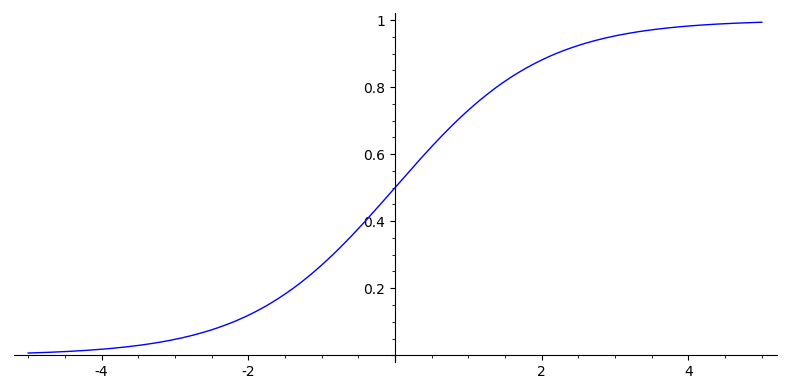
\includegraphics[width=10cm]{sigmoide.png} $$
Observamos que para $x$ "grandes" la función es un muy plana y por lo tanto $f'(x)$ será prácticamente nula. Esto hace que para algunos $z_i^{(c-1)}$ tanto $\frac{\partial C_E}{\partial \omega} $ como $\frac{\partial C_E}{\partial b} $ sean muy bajos y por lo tanto la red aprenda muy lento. Por lo tanto un desearía tener una función de coste $C$ tal que
$$\frac{\partial C}{\partial \omega^{(c-1)}_{ji}}=(a_i^{(c)}-s_i)\cdot a_i^{(c-1)} $$
$$\frac{\partial C}{\partial u^{(c-1)}_i}=(a_i^{(c)}-s_i) $$
es decir, sin el factor $f'(z_i) $. Observamos que para una función de coste cualquiera $C$ tenemos, por la regla de la cadena, que
$$\frac{\partial C}{\partial u^{(c-1)}_i}=\frac{\partial C}{\partial a_i^{(c)}}\frac{\partial a_i^{(c)}}{\partial z^{(c-1)}_i}\frac{\partial z_i^{(c-1)}}{\partial u^{(c-1)}_i}=\frac{\partial C}{\partial a_i^{(c)}}f'(z_i^{(c-1)})\cdot 1 $$
Como la sigmoide cumple $f'(x)=f(x)(1-f(x)) $ entonces
$$\frac{\partial C}{\partial u^{(c-1)}_i}=\frac{\partial C}{\partial a_i^{(c)}}f(z_i^{(c-1)})(1-f(z_i^{(c-1)}))=\frac{\partial C}{\partial a_i^{(c)}}a_i^{(c)}(1-a_i^{(c)}) $$
Por otro lado queríamos que $C$ cumpliera
$$\frac{\partial C}{\partial u^{(c-1)}_i}=(a_i^{(c)}-s_i) $$
por lo tanto
$$(a_i^{(c)}-s_i)=\frac{\partial C}{\partial a_i^{(c)}}a_i^{(c)}(1-a_i^{(c)}) $$
Denotando $a\equiv a_i^{(c)}$ e integrando
$$C=\int \frac{\partial C}{\partial a} da=\int \frac{a-s_i}{a(1-a)} da= -\left(s_i\ln{a}+(1-s_i)\ln{(1-a)}\right)$$
Observamos que si $a\in(0,1) $ entonces el logaritmo es negativo y con el signo del principio tendremos que $C>0$.\\

Además observamos que si $s_i=0$ y $a\approx 0$ (lo cual es bueno) entonces $\ln(1-a)\approx 0 $ y por lo tanto el "coste" será mínimo. Por otro lado si $s_i=1$ y $a\approx 1$ entonces $\ln(a)=0$ y de nuevo el coste es mínimo.\\

De modo que esta nueva función de coste tiene la ventaja respecto la $C_E$ de que no se ralentiza su aprendizaje debido a $f'(z_i)$.\\

Por lo general conoceremos a
$$C=-\frac{1}{n}\sum_x\left(y\ln{a}+(1-y)\ln{(1-a)}\right) $$
como the Cross-entropy cost function.\\

\end{document}


%\href{http://neuralnetworksanddeeplearning.com/}\\
%\href{https://github.com/mnielsen/neural-networks-and-deep-learning/blob/master/src/network.py}\\
%\href{http://colah.github.io/posts/2015-08-Backprop/}



\begin{coment}
\section*{Descenso del gradiente}
\paragraph{Método de minimizar el gradiente}
El error del algoritmo tiene que pensarse como una función $f$ que depende de los parámetros $\omega_i$ y $u_i$.\\
Esa función $f$ dependerá de demasiadas variables como para resolver $\nabla f=0 $. De hecho no sería ni siquiera lo ideal ya que tras cada entreno seguiremos corrigiendo los pesos etc.\\

La fórmula recursiva que usaremos es 
$$\omega_{i}=\omega_i-\alpha\frac{\partial f}{\partial \omega_i} $$
cada una de los pesos $\omega_i $ se modificará de esta forma. El signo $-$ es debido a que un mínimo relativo de una función $f$ esta en el sentido contrario de la derivada y el coeficiente real $\alpha $ es debido a que si no puede entrar en bucle el algoritmo o que la corrección puede ser demasiado brusca, únicamente nos importa que $\omega_i$ se modifique en el sentido $-\frac{\partial f}{\partial \omega_i} $. El valor de $\alpha$ suele estar entre $0.1 $ y $0.01$.\\

La red tendrá $c$ capas y cada capa tendrá $n_k$ neuronas $1\leq k\leq c $. Cada neurona está conectada con cada una de las neuronas de la siguiente capa.\\
La conexión de la $i$-ésima neurona $1\leq i\leq n_k$ de la capa $k$ con la neurona $j$-ésima $1\leq j\leq n_{k+1}$ de a capa $k+1$ la denotaremos por $\omega^{(k)}_{ij} $\\

A la práctica lo que haremos será hacer media de los errores de unas cuantos ejemplos y modificaremos los pesos y umbrales en funcion de esa media.\\
Esto se conoce como descenso del gradiente estocástico. La fórmula quedaría así
$$f=\frac1{2n}\sum{f_i} $$
donde $f_i$ es el error de caca uno de los $n$ pruebas.\\

Además el error de cada prueba se calculará como el cuadrado de la diferencia de lo experimental y lo esperado.

\section*{Backpropagation}
\paragraph{Sigmoide y output de una neurona}
\textcolor{red}{Se dice que ahora se usa mejor la función ReLU$(x)=$max$(0,x) $}.\\
$$f(x)=\frac1{1+e^{-x}}\in (0,1) $$
y cumple que 
$$f'(x)=f(x)\cdot (1-f(x)) $$

A cada neurona le llegan inputs $z_i$ con pesos $\omega_i$ respectivamente. Además también tendrá como input un umbral $u$.\\
El output $a$ de cada neurona será
$$a=f(u+\sum w_iz_i) $$
donde $f$ es la sigmoide

$$\frac{\partial a}{\partial u}=\frac{\partial f}{\partial (u+\sum w_iz_i)}\cdot \frac{\partial (u+\sum w_iz_i)}{\partial u}=\frac{\partial f}{\partial u}=a\cdot (1-a) $$
$$\frac{\partial a}{\partial \omega_j}=\frac{\partial f}{\partial (u+\sum w_iz_i)}\cdot \frac{\partial (u+\sum w_iz_i)}{\partial \omega_j}=\frac{\partial f}{\partial u}=a\cdot (1-a)\cdot z_j $$

Por lo general al output de la neurona $i\leq n_k$ de la capa $k$ le llamaremos $a^{(k)}_i$.\\
El output de la capa $k=1$ es simplemente el input del programa.\\
Por lo tanto para $k>1$ (y siguiendo la notación inicial general), el output de la neurona $i\leq n_k$ de la capa $k$ es
$$a^{(k)}_i=f(u^{(k)}_i+\sum_{j=1}^{n_{k-1}} w^{(k-1)}_{ji}z_j) $$
donde $z_i$ son los outputs de las $n_{k-1}$ neuronas de la capa $k-1$ por lo tanto también lo podemos escribir como
$$a^{(k)}_i=f(u^{(k)}_i+\sum_{j=1}^{n_{k-1}} w^{(k-1)}_{ji}a^{(k-1)}_j) $$

Por lo general podemos pensarlo como \\
\textcolor{red}{creo k me he colado con la capa de las $\omega$,deberia ser k y no k-1}
$$a^{(k)}=f\left(
\begin{pmatrix}
w^{(k-1)}_{11} & w^{(k-1)}_{12} \cdots w^{(k-1)}_{1n}\\
w^{(k-1)}_{21} & w^{(k-1)}_{22} \cdots w^{(k-1)}_{2n}\\
\vdots   & \ddots  \\
w^{(k-1)}_{m1} & w^{(k-1)}_{m2} \cdots w^{(k-1)}_{mn}\\
\end{pmatrix} 
\begin{pmatrix}
a^{(k-1)}_1 \\
a^{(k-1)}_2 \\
\vdots \\
a^{(k-1)}_n \\
\end{pmatrix}
+
\begin{pmatrix}
u^{(k)}_1 \\
u^{(k)}_2 \\
\vdots \\
u^{(k)}_n \\
\end{pmatrix}\right)$$
y por lo tanto en forma matricial nos quedaría
$$a^{(k)}=f(\omega^{(k-1)}a^{(k-1)}+u^{(k)}) $$

\paragraph{Algoritmo de propagación hacia atrás (Backpropagation)}
Sea $c$ el número de capas. Los outputs $a^{(c)}_i$ de las $n_c$ neuronas de la última capa son los outputs del algoritmo. A estos outputs también les llamaremos $y_l$, $l\leq n_c $.\\
Para calcular la variación de output $y_l$ del algoritmo con respecto de cada $\omega^{(k)}_{ij} $ vemos que como
$$y_i=f(u^{(c)}_i+\sum_{j=1}^{n_{c-1}} w^{(c-1)}_{ji}a^{(c-1)}_j) $$
entonces
$$\frac{\partial y_l}{\omega^{(k)}_{ij} }=\frac{\partial y_l}{u^{(c)}_i+\sum_{j=1}^{n_{c-1}} w^{(c-1)}_{ji}a^{(c-1)}_j}\cdot\frac{u^{(c)}_i+\sum_{j=1}^{n_{c-1}} w^{(c-1)}_{ji}a^{(c-1)}_j}{\omega^{(k)}_{ij} } $$
vemos que 
$$\frac{\partial y_l}{u^{(k)}_i+\sum_{j=1}^{n_{k-1}} w^{(k-1)}_{ji}a^{(k-1)}_j}=y_l\cdot (1-y_l) $$
$$\frac{u^{(c)}_i+\sum_{j=1}^{n_{c-1}} w^{(c-1)}_{ji}a^{(c-1)}_j}{\omega^{(k)}_{ij} }=w^{(c-1)}_{ji}\sum \frac{\partial a^{(c-1)}_j}{\partial \omega^{(k)}_{ij}} $$

Sean $s_i$ lo valores deseados y $y_i$ los outputs del algortimo entonces consideraremos el error 
$$e=E(y_i)=\frac1{2}\sum (y_i-s_i)^2 $$
Observamos que minimizar este error es equivalente a minimizar la distancia euclidiana entre puntos.\\

Los inputs y outputs del algoritmo tienen que estar del 0 al 1.\\

Denotaremos $z^l_j=\sum_k \omega^l_{jk}a^{l-1}+b_j^l $ de manera que simplemente $a^l_j=f(z^l_j) $ y en forma matricial tendremos
$$z^l=\omega^la^{l-1}+b^l \ a^l=f(z^l) $$
Denotaremos el error de $z_j^l$ como 
$$\delta_j^l=\frac{\partial C}{\partial z_j^l} $$
y como siempre denotaremos por $\delta^l$ el vector de errores asociados con la capa $l$.\\
Observamos que
$$\delta^l_j=\frac{\partial C}{\partial a^l_j}\frac{\partial a_j^l}{\partial z_j^l}=(a^l_j-y_j)\cdot f'(z_j^l) $$
En notación matricial tendremos
$$\delta^l=
\left(
\begin{array}{c}
\frac{\partial C}{\partial a^l_1}\\
\vdots\\
\frac{\partial C}{\partial a^l_n}

\end{array}\right)
\odot\left(
\begin{array}{c}
f'(z_1^l)\\
\vdots\\
f'(z_n^l)
\end{array}\right)
=\nabla_{a^l}C\odot f'(z^l)
=(a^l-y)\odot f'(z^l)$$

donde $\odot$ representa el producto de Hadamard, es decir, el producto componente a componente.\\

Ahora encontraremos una fórmula para expresar el error de la capa $l$ $(\delta^l) $ en función del error de la capa $l+1$ $(\delta^{l+1}) $. Como
$$z_k^{l+1}=\sum_{j}\omega_{kj}^{l+1}a^l_j+b_k^{l+1}=\sum_{j}\omega_{kj}^{l+1}f(z^l_j)+b_k^{l+1} $$
entonces derivando obtenemos
$$\frac{\partial z_k^{l+1}}{\partial z_j^l}=\omega_{kj}^{l+1}f'(z_j^l) $$

$$\delta_j^l=\frac{\partial C}{\partial z_j^l}=\sum_k \frac{\partial C}{\partial z_j^{l+1}}\frac{\partial z_j^{l+1}}{\partial z_j^l}=\sum_k\delta_k^{l+1}\frac{\partial z_j^{l+1}}{\partial z_j^l}=\delta_k^{l+1}\omega_{kj}^{l+1}f'(z_j^l) $$
y en notación matricial
$$\delta^l=((\omega^{l+1})^T\delta^{l+1})\odot f'(z^l) $$
$$\frac{\partial C}{\partial b_j^l}=\frac{\partial C}{\partial z_j^l}\frac{\partial z_j^l}{\partial b_j^l}=\delta_j^l\cdot 1=\delta_j^l $$
$$\frac{\partial C}{\partial \omega_{jk}^l}=\frac{\partial C}{\partial \omega_{jk}^l}\frac{\partial \omega_{jk}^l}{\partial b_j^l}=\delta_j^l\cdot a_k^{l-1} $$

\end{coment}











